\documentclass{article}
\usepackage[utf8]{inputenc}
\usepackage[a4paper, top=3cm, bottom=3cm, left=3cm, right=3cm]{geometry}
\usepackage{amsmath}
\usepackage{amsthm}
\usepackage{amssymb}
\usepackage{fancyhdr}
\usepackage{hyperref}
\usepackage{graphicx}
\usepackage{subfig}
\usepackage[T1]{fontenc}    % https://tex.stackexchange.com/questions/453540/

\pagestyle{fancy}
\fancyhf{}
\lhead{Competitive Programming}
\rhead{Week-1}
\cfoot{\thepage}

\newcommand{\B}[1]{\textbf{#1}}
\newcommand{\I}[1]{\textit{#1}}
\newcommand{\T}[1]{\texttt{#1}}

\title{\textbf{SoC 2023: Competitive Programming \\ {\Large Week-1: Basics and C++ STL}}}
\author{Mentor: Virendra Kabra}
\date{Summer 2023}

\begin{document}
\begin{sloppypar}       % for overfull, etc.

    \maketitle
    \tableofcontents
    \thispagestyle{empty}

    \newpage
    % \setcounter{page}{1}

    \section{Resources}
    \begin{itemize}
        \item Competitive Programming: Need to solve small problems in a limited time. Most of these are based on standard concepts that we are going to cover. For acceptance, solutions must adhere to a specified time-limit and memory-limit.
        \item Online Platforms for contests and practice: Codeforces, Codechef, AtCoder, SPOJ, CSES, etc. We would mainly do problems from Codeforces and CSES Problem Set.
        \begin{itemize}
            \item Can filter questions on specific topics or rating levels on Codeforces
            \item CSES has topic-wise sets
        \end{itemize}
        \item References:
        \begin{itemize}
            \item CP: Competitive Programmer's Handbook (CSES) by Antti Laaksonen, \href{https://cp-algorithms.com/}{cp-algorithms}, Competitive Programming by Steven and Felix Halim, blogs on Codeforces and other websites
            \item Theoretical DSA: CLRS, Kleinberg-Tardos
        \end{itemize}
        \item Most programmers use C++ for smaller execution time and a convenient template library. Some use Python, Java, etc.
    \end{itemize}

    \newpage

    \section{Basics}

    \subsection{Template}
    \begin{itemize}
        \item \href{run:../programs/1_template.cpp}{Starting Template}
        \item Get VSCode to identify the path to \verb|bits/stdc++.h|: \href{https://www.youtube.com/watch?v=pyn0TjUnf18}{YT Link}
        \item \href{https://code.visualstudio.com/docs/editor/userdefinedsnippets}{VSCode user snippets}
        \item \verb|ios_base::sync_with_stdio(false); cin.tie(0);|\\
        disables synchronization between streams and unties \verb|cin| from \verb|cout|. Buffering \verb|cout| has a side-effect of speed improvement.
        \item \verb|"\n"| vs \verb|endl|\\
        \verb|endl| flushes the output. Use \verb|"\n"| for better execution speed. \href{https://codeforces.com/blog/entry/45307}{Interactive Questions} require flushing of output buffer. Use \verb|cout.flush()| and the like.
        \item \href{https://codeforces.com/blog/entry/61587}{Random numbers}
        \item File read and write for debugging and testing
        \item \verb|define| macros and \verb|typedef|s
        \item \verb|long long|, \verb|unsigned long long|
    \end{itemize}

    \subsection{Time Complexity}
    \begin{itemize}
        \item Big-O Notation: On a high level, keep the dominant (faster growing) term in a function to get the ``order'' with which it grows. Constant factors are ignored. Examples:
        \begin{itemize}
            \item $3n^2 + 2n + 5 = O(n^2)$. Grows like $n^2$
            \item $n + \log{n} = O(n)$, as $n$ grows faster than $\log{n}$
            \item $f(n) = 10^{100}n$ is $O(n)$ and $g(n) = n^2$ is $O(n^2)$. However, for all practical purposes, $g$ is faster
        \end{itemize}
        \item Go through \href{https://codeforces.com/blog/entry/104888}{this CF blog post} or Chapter-2 of the Handbook. It has examples on how to compute time-complexity in terms of the inputs.
        \item Constraints would be mentioned in the problem: with C++, roughly $10^6-10^7$ operations/second. So if $n\le 10^5$ and time limit $\le 1$ second, then $O(n^2)$ won't work (TLE). If $n\le 20$, then brute force ($2^n$) might work.
    \end{itemize}

    \subsection{Operators}
    \begin{itemize}
        \item Commonly used \I{bitwise} operators \T{|, \&, \~{}, <<, >>, \^{}}
        \item \href{https://www.geeksforgeeks.org/operators-in-c/}{GFG Reference}
        \item XOR
        \begin{itemize}
            \item Exclusive OR: \T{0\^{}0=0, 1\^{}1=0, 0\^{}1=1, 1\^{}0=1}
            \item \T{p\^{}0 = p, p\^{}(1\dots1) = \~{}p, p\^{}\~{}p = 1\dots1}. Note that \T{1\dots1} is -1 in 2's complement notation
            \item XOR is associative and commutative
        \end{itemize}
    \end{itemize}

    \newpage

    \section{C++ STL Data Structures}

    Some commonly used data structures with their methods.
    \begin{enumerate}
        \item \T{vector}
        \begin{itemize}
            \item Dynamic length array. Memory for elements is contiguously allocated on heap
            \item \href{https://www.geeksforgeeks.org/vector-in-cpp-stl/}{GFG Reference} for methods and respective time-complexities. Constant-time access, linear-time insertion and deletion. Insertion at the end is \I{amortized} constant-time.
            \item \href{run:../programs/2_vector.cpp}{File}
        \end{itemize}
        \item \T{string}
        \begin{itemize}
            \item Dynamic \T{char} array. Many convenient STL functions
            \item \href{https://www.geeksforgeeks.org/stdstring-class-in-c/}{Methods}
            \item \href{run:../programs/3_string.cpp}{File}
        \end{itemize}
        \item \T{stack}, \T{queue}, \T{deque}, \T{priority\_queue} \T{list}. Images from GFG
        \begin{itemize}
            \item Stack: Last-In-First-Out
            \item Queue: First-In-First-Out
            \begin{center}
                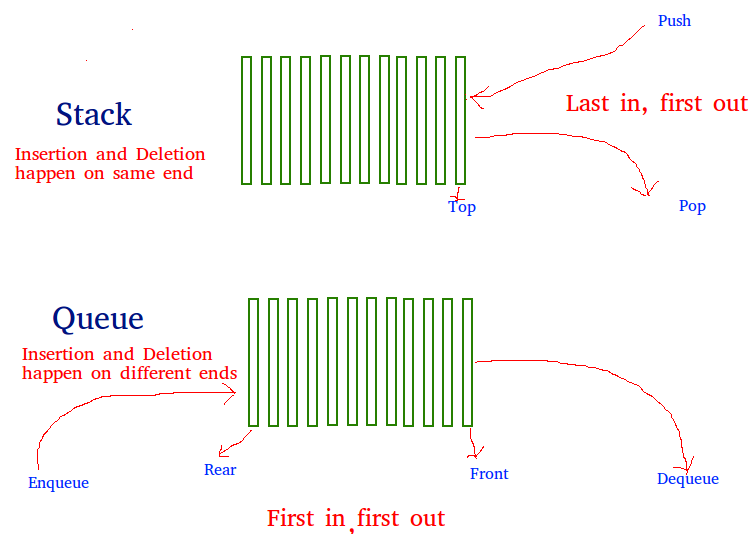
\includegraphics[width = 0.9\linewidth]{../images/1_Stack-Queue.png}
                % \captionof{figure}{}
            \end{center}
            \item Double Ended Queue: Allows insertions and deletions from either end
            \item Priority Queue: Top of queue is greatest/least (or custom comparison criteria)
            \begin{center}
                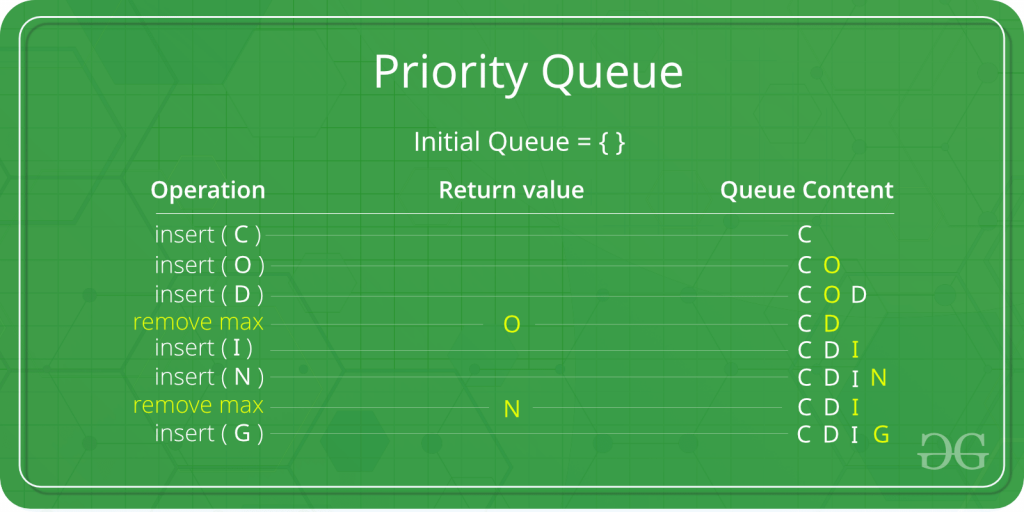
\includegraphics[width = 0.8\linewidth]{../images/2_Priority-Queue.png}
            \end{center}
            \item List: Similar to \T{vector}, but with non-contiguous memory allocation. This allows constant-time insertions and deletions, but slower access.
            \item Methods and time-complexities: \href{https://www.geeksforgeeks.org/stack-in-cpp-stl/}{stack}, \href{https://www.geeksforgeeks.org/queue-cpp-stl/}{queue}, \href{https://www.geeksforgeeks.org/priority-queue-in-cpp-stl/}{priority queue}, \href{https://www.geeksforgeeks.org/deque-cpp-stl/}{deque}, \href{https://www.geeksforgeeks.org/list-cpp-stl/}{list}
            \item \href{run:../programs/4_stack-queue-pq.cpp}{File}
        \end{itemize}
        \item \T{pair}, \T{map}, \T{set}
        \begin{itemize}
            \item Pair: Two elements, \T{first} and \T{second}. For example, \T{\{int, vector<int>\}}
            \item Set: Collection of elements. Similar to \T{vector}, but faster lookups, deletes. For example, \T{\{-5,0,3\}}
            \begin{itemize}
                \item Ordered: Elements are ordered by some comparator. For example, default is ascending order for an ordered set of \T{int}s.
                \item Unordered: Not ordered, allowing faster inserts, lookups, deletions. However, time-complexity constants might be higher.
                \item STL: \T{set} and \T{unordered\_set}
            \end{itemize}
            \item Map: Key-value \T{pair}s. For example, \T{map<int, unsigned int>} with entries \T{\{\{-5, 5\}, \{1, 0\}, \{20, 10\}\}}.\\
            Similar to sets, we have ordered and unordered maps: \T{map} and \T{unordered\_map}. Ordering is done by keys.
            \begin{center}
                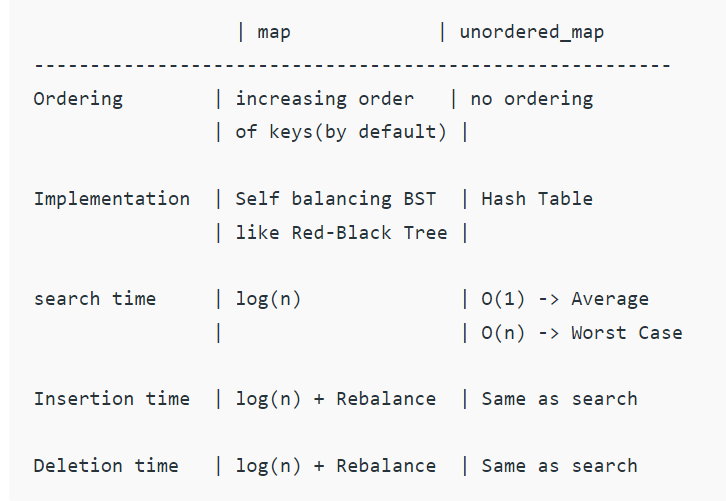
\includegraphics[width = 0.9\linewidth]{../images/3_map-vs-umap.png}
            \end{center}
            \item A popular question: Given an array of integers and a target sum, is there a pair that add up to the target sum?\\
            $O(n^2), O(n\log{n}), O(n)$
            \item \href{run:../programs/5_map-set.cpp}{File}
        \end{itemize}
        \item Bitset. \href{run:../programs/6_operators.cpp}{File}
    \end{enumerate}

    \section{Todos}
    \begin{itemize}
        \item Visit links in this document
        \item Start out with Chapters 1 and 4 of the CP handbook
        \item CSES Introductory Problems
    \end{itemize}

\end{sloppypar}
\end{document}